\section{Activity: Rubber Band Instrument}
\subsection{Materials required}
\begin{enumerate}
\item Rubber bands
\item Geometry box or pencil box
\item Two pens or pencils
\end{enumerate}
\subsection{Procedure}
Close the geometry box or pencil box. Stretch a rubber band around the box so that it lies across the top surface. Place a pen or pencil under the rubber band near one end of the box. Place another pen or pencil under the rubber band near the other end of the box. This will lift the rubber band slightly above the surface of the box. See Figure 3. Pluck the rubber band with your finger.
\begin{marginfigure}
  \centering
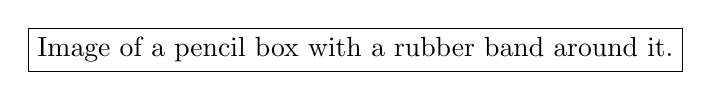
\begin{tikzpicture}
    \node[draw] at (0,0) {Image of a pencil box with a rubber band around it.};
  \end{tikzpicture}
  \caption{\label{rubberbox}Pencil box with rubber band around it.}
\end{marginfigure}
\newthought{Observe} the movement of the rubber band. Do you hear a sound? What part of the setup is moving?